\chapter{Desenvolvimento}
\label{c_desenvolvimento}

Este capítulo apresenta a interface desenvolvida, denominada de RoPE AR. Primeiramente a \autoref{sec:elementos_interface} descreve a interface do ponto de vista do usuário, ou seja, os elementos com os quais a criança ou o adulto interagem. A seguir a \autoref{sec:detalhes_tecnicos} traz detalhes técnicos das tecnologias utilizadas, como a comunicação Bluetooth entre smartphone e robô.

\section{Elementos da interface}
\label{sec:elementos_interface}
\subsection{Aplicativo}
A interação inicial ocorre quando um adulto usa o aplicativo para conectar o smartphone com o RoPE. Ele é constituído de apenas duas telas. A primeira tela permite conectar o smartphone ao brinquedo (\autoref{fig:app_connection}). Ela mostra um desenho do RoPE e uma lupa indicando a procura pelo brinquedo, ou seja, a conexão com o brinquedo físico. Gravações de uma voz guiam o usuário para que ligue o RoPE acionando seu botão inferior e informam quando a conexão foi estabelecida. Ao se conectar o brinquedo também emite um \textit{feedback} sonoro e luminoso como \i{feedback}.

\begin{figure}[!h]
    \begin{subfigure}{.5\textwidth}
        \centering
        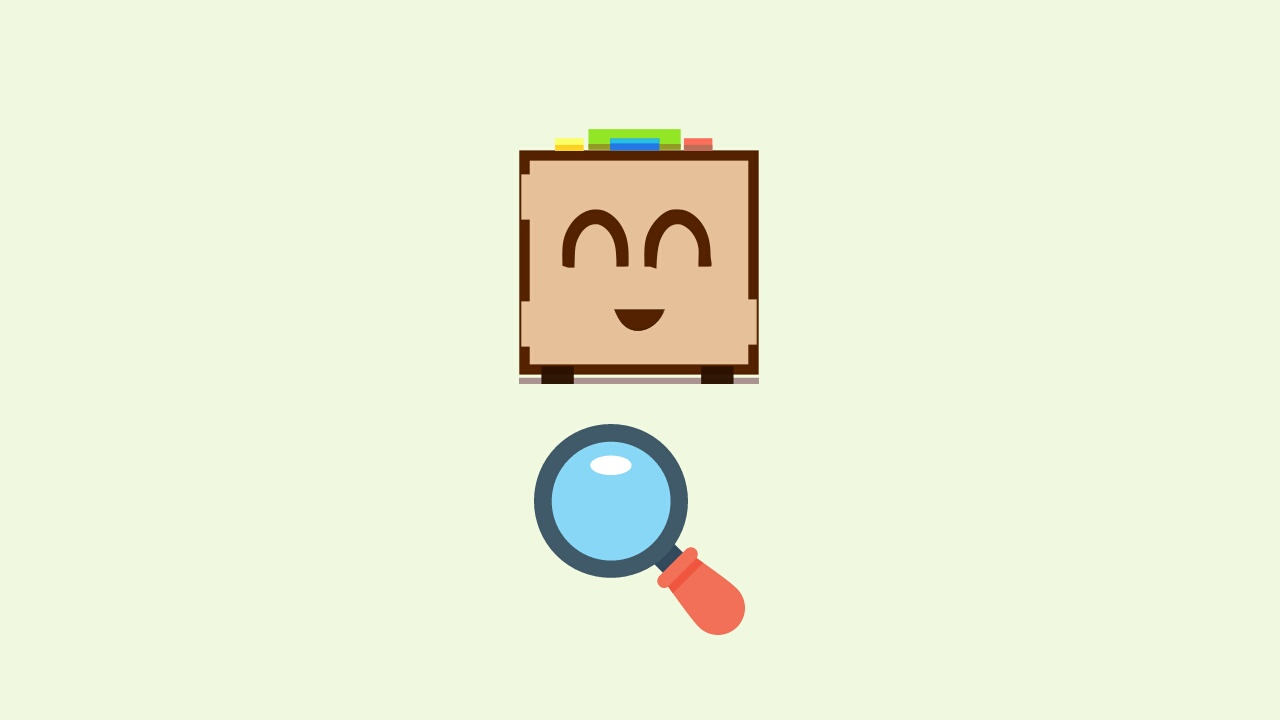
\includegraphics[width=.9\linewidth,fbox]{figs/app_connection.jpeg}
        \caption{Tela de conexão.}
        \label{fig:app_connection}
    \end{subfigure}
    \begin{subfigure}{.5\textwidth}
        \centering
        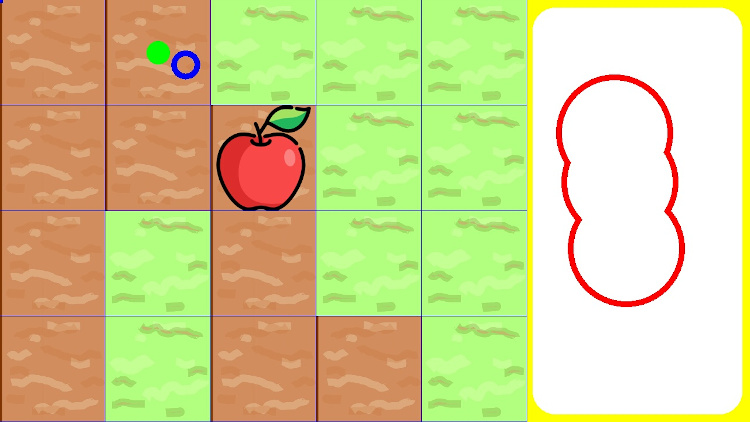
\includegraphics[width=.9\linewidth,fbox]{figs/app_game.jpeg}
        \caption{Tela de desafio.}
        \label{fig:app_game}
    \end{subfigure}
    \caption{Telas do aplicativo.}
    \label{fig:app_screens}
\end{figure}

A segunda tela aparece após a conexão com o brinquedo. Ela apresenta um desafio contendo uma sequência de mapas (\autoref{fig:app_game}). Cada mapa tem um caminho, uma posição inicial (circulo verde) e um ou mais itens coletáveis. Na direita da tela há um retângulo branco. Ao ser projetada, a cor branca não interfere nas características visuais dos blocos físicos. Manter essas características auxilia na identificação das marcas fiduciais. Por fim, o último elemento da tela são círculos vermelhos que indicam quais blocos fazem parte do algoritmo a ser executado pelo brinquedo. 

Relembrando, a criança não interage com o aplicativo. Toda interação ocorre com o RoPE e com blocos físicos, posicionados no chão. A criança cria algoritmos ao sequenciar os blocos físicos, que são identificados pelo App. Caso exista um algoritmo válido, a luz emitida pelo projetor destaca os blocos do algoritmo.

O brinquedo executa o algoritmo quando a criança pressiona seu botão verde. Ao executar o programa, o brinquedo se move e o aplicativo capta as posições percorridas. Deste modo, consegue identificar se o brinquedo colidiu ou não nos itens coletáveis do mapa. Quando o brinquedo coleta todos os itens, o aplicativo reproduz uma gravação de parabenização, e mostra o mapa seguinte. Caso não existam outros mapas, uma gravação sinaliza que a brincadeira acabou.

\subsection{Elementos tangíveis}
A interface possui quatro tipos de elementos tangíveis: o brinquedo RoPE, os blocos de código, os marcadores de calibragem, e o ativador de depuração  (\autoref{fig:tangible_elements}).
\begin{enumerate}
\item \textbf{Brinquedo RoPE}: Ao brinquedo foi adicionada uma marca fiducial para que seja identificada sua posição. A informação da posição do brinquedo permite à interface reagir a seus movimentos, disparando eventos sonoros e animações. Além da marca fiducial, o brinquedo tem os botões superiores. Por meio do botão verde do brinquedo a criança inicia a execução do algoritmo programado com os blocos de papelão. Os demais botões são usados no modo de depuração. Neste modo, o brinquedo para antes de cada movimento e acende a seta indicando qual será a próxima ação. O brinquedo continua a execução quando o botão é clicado, e assim a criança pode observar a execução passo a passo.
\item \textbf{Blocos de código}:  Há dois tipos de blocos: os direcionais e o bloco de início. Os blocos direcionais tem desenhos que mostram o RoPE fazendo o movimento de andar pra frente, andar para trás, virar a esquerda, e virar à direita. Há também o bloco de início, que corresponde ao botão verde do RoPE e indica o início da execução. Os blocos direcionais devem ser encaixados no bloco de início, formando uma sequência. O formato curvado busca sugerir como deve ser o encaixe entre os blocos. O bloco de início  tem a parte inferior reta para impedir o encaixe de outros blocos incorretamente.
\item \textbf{Marcadores de calibragem}: Marcas fiduciais que identificam os quatro cantos da área projetada. Para projetar os elementos na posição correta o algoritmo precisa mapear a posição de projeção, bem como identificar a distorção de perspectiva resultante. Um adulto responsável por preparar a interface coloca os marcadores nos cantos da área projetada, e a câmera do \textit{smartphone} capta a posição da mesma. Após a captação os marcadores são retirados.
\item \textbf{Ativador de depuração}: O quarto elemento tangível é representado por uma joaninha (em inglês \textit{ladybug}. Essa figura foi selecionada por ser uma figura lúdica e também por ser um inseto, uma referência à origem do termo \textit{bug}. Quando a joaninha está visível o brinquedo RoPE entra em modo de depuração, no qual a execução de cada comando exige que a criança aperte o botão correspondente. Quando não está visível, o brinquedo executa a sequência completa de comandos sem interrupção.
\end{enumerate}

\begin{figure}
\centering
        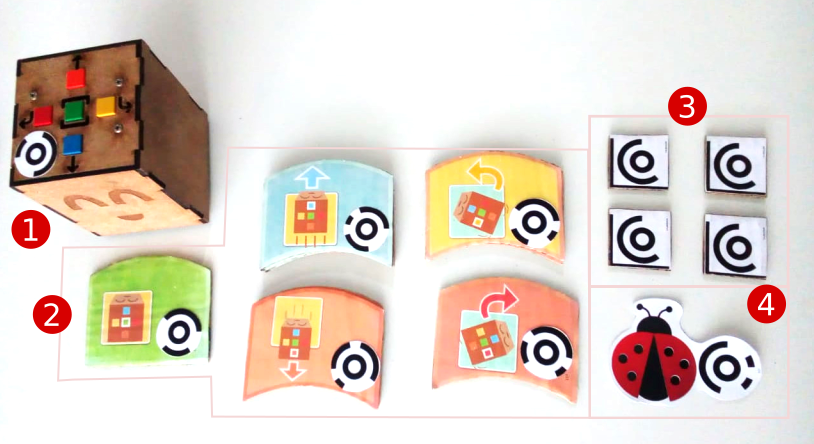
\includegraphics[width=.9\linewidth,fbox]{figs/tangible_elements.png}
        \caption{Elementos tangíveis. 1 - RoPE. 2 - Blocos de código. 3 - Marcadores de calibragem. 4 - Ativador de depuração.}
        \label{fig:tangible_elements}
\end{figure}
Todos os elementos tangíveis possuem marcas fiduciais de 4cm de diâmetro. Essa medida foi utilizada para facilitar a identificação das mesmas por uma câmera capaz que gera imagens de 1280x720 pixeis durante gravação de vídeo. Essa medida foi obtida de forma empírica, iniciando com 3 cm de diâmetro e aumentando o tamanho até a identificação de todas as marcas presentes no campo de visão da câmera. Um último detalhe é que as marcas são impressas em papel cartão pois este não reflete luz, o que prejudica a captação das marcas.

\section{Aspectos técnicos}
\label{sec:detalhes_tecnicos}
\subsection{Arquitetura}
A arquitetura do projeto possui quatro dispositivos: um smartphone, o brinquedo RoPE, um servidor web e um projetor (\autoref{fig:system_overview}). Estes dispositivos se comunicam por meio de conexão sem fio. Nesta comunicação os dados enviados são as ações executadas pelo brinquedo e as imagens a serem mostradas no tapete.  A seções seguintes apresentam cada um destes componentes.

\begin{figure}[!h]
    \centering
    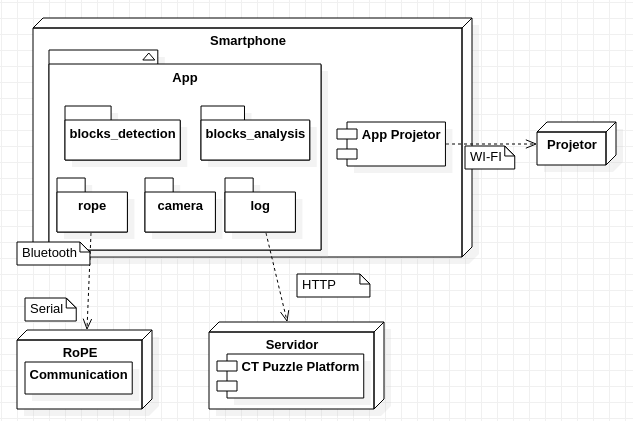
\includegraphics[width=.8\linewidth,fbox]{figs/system_overview.png}
    \caption{Visão geral dos componentes do sistema.}
    \label{fig:system_overview}
\end{figure}

\subsubsection{Smartphone}
Um smartphone com sistema operacional Android é o componente central, pois coordena a comunicação com o projetor e o servidor web. Dois aplicativos permanecem ativos no smartphone. O primeiro aplicativo é o Mirroring 360, que transmite a tela do smartphone ao projetor via Wi-Fi. Esse aplicativo está disponível na loja de aplicativos da Google, e há diversos aplicativos similares que executam a mesma função. O Mirroring 360 foi selecionado por ser gratuito e não mostrar anúncios.

O segundo aplicativo foi desenvolvido neste trabalho. Ele tem as funções de:
\begin{itemize}
    \item gerar o cenário virtual
    \item captar os blocos tangíveis e, se houver um algoritmo, enviá-lo ao RoPE
    \item detectar colisões entre o RoPE e os elementos virtuais coletáveis
    \item enviar os eventos ocorridos para a CtPuzzle Platform
\end{itemize}

Para isso, o aplicativo é dividido em cinco módulos: Câmera, Detecção de blocos, Análise dos blocos, Registro de interações, e Comunicação com o RoPE . As próximas seções seções apresentam detalhes de implementação destes módulos.

%\begin{figure}
%    \centering
%    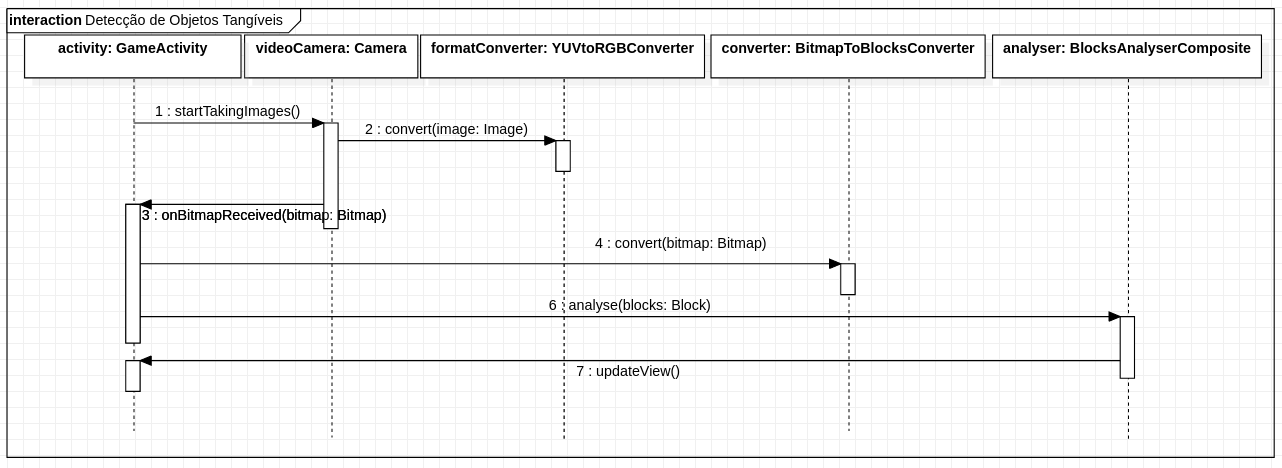
\includegraphics[width=0.95\textwidth,fbox]{figs/sequence_diagram.png}
%    \caption{Diagrama de sequência: obtenção de imagem, identificação dos topcodes e análise dos elementos tangíveis.}
%    \label{fig:sequence_diagram}
%\end{figure}

\subsubsubsection{Módulo de Câmera}
\label{sec:camera}

%O diagrama de sequência da \autoref{fig:sequence_diagram} mostra classes desses módulos sendo invocadas. O controle principal solicita o início da captação de imagens, que utiliza conversão de formato YUV para RGB (explicado na \autoref{sec:camera}). Depois da obtenção de imagem, ocorre a identificação dos objetos tangíveis presentes na cena. Por fim ocorre a análise do posicionamento dos objetos para gerar feedbacks visuais.

A câmera capta as imagens utilizadas na identificação dos elementos tangíveis, com os quais a criança interage. Para essa captação o sistema operacional Android oferece dois modos de acesso à câmera: fotografia e vídeo. O modo fotografia obtém imagens com mais resolução, porém imagens maiores também precisam de mais tempo de processamento \footnote{O tempo entre captura e processamento ficou entre 0.5 a 1 segundo no modo fotografia. Essa medição ocorreu por meio de logs com o dispositivo M5c.}. O modo vídeo obtém um fluxo contínuo de imagens, porém em menor resolução. Esta pesquisa usou dois smartphones: um Meizu M5c e um Xiaomi Redmi 8. A \autoref{fig:photo_video_dimensions} mostra, em proporção, as resoluções disponíveis para os dois smartphones utilizados.

% {\renewcommand{\arraystretch}{1.5}
    
%     \begin{table}[!h]
%         \begin{tabular}{|l|c|c|} \hline
%         Modelo         	   & Resolução de foto & Resolução de vídeo (pixeis) \\ \hline
%         Meizu M5C          & 3264 x 2448       & 1280 x 720  \\ \hline
%         Xiaomi Redmi 8     & 4032 x 3016       & 1920 x 1080 \\ \hline
%         \end{tabular}
%         \caption{Resolução de câmera dos smartphones utilizados.}
%         \label{tab:resolutions}
%     \end{table}   
% }

\begin{figure}[!h]
   \centering
   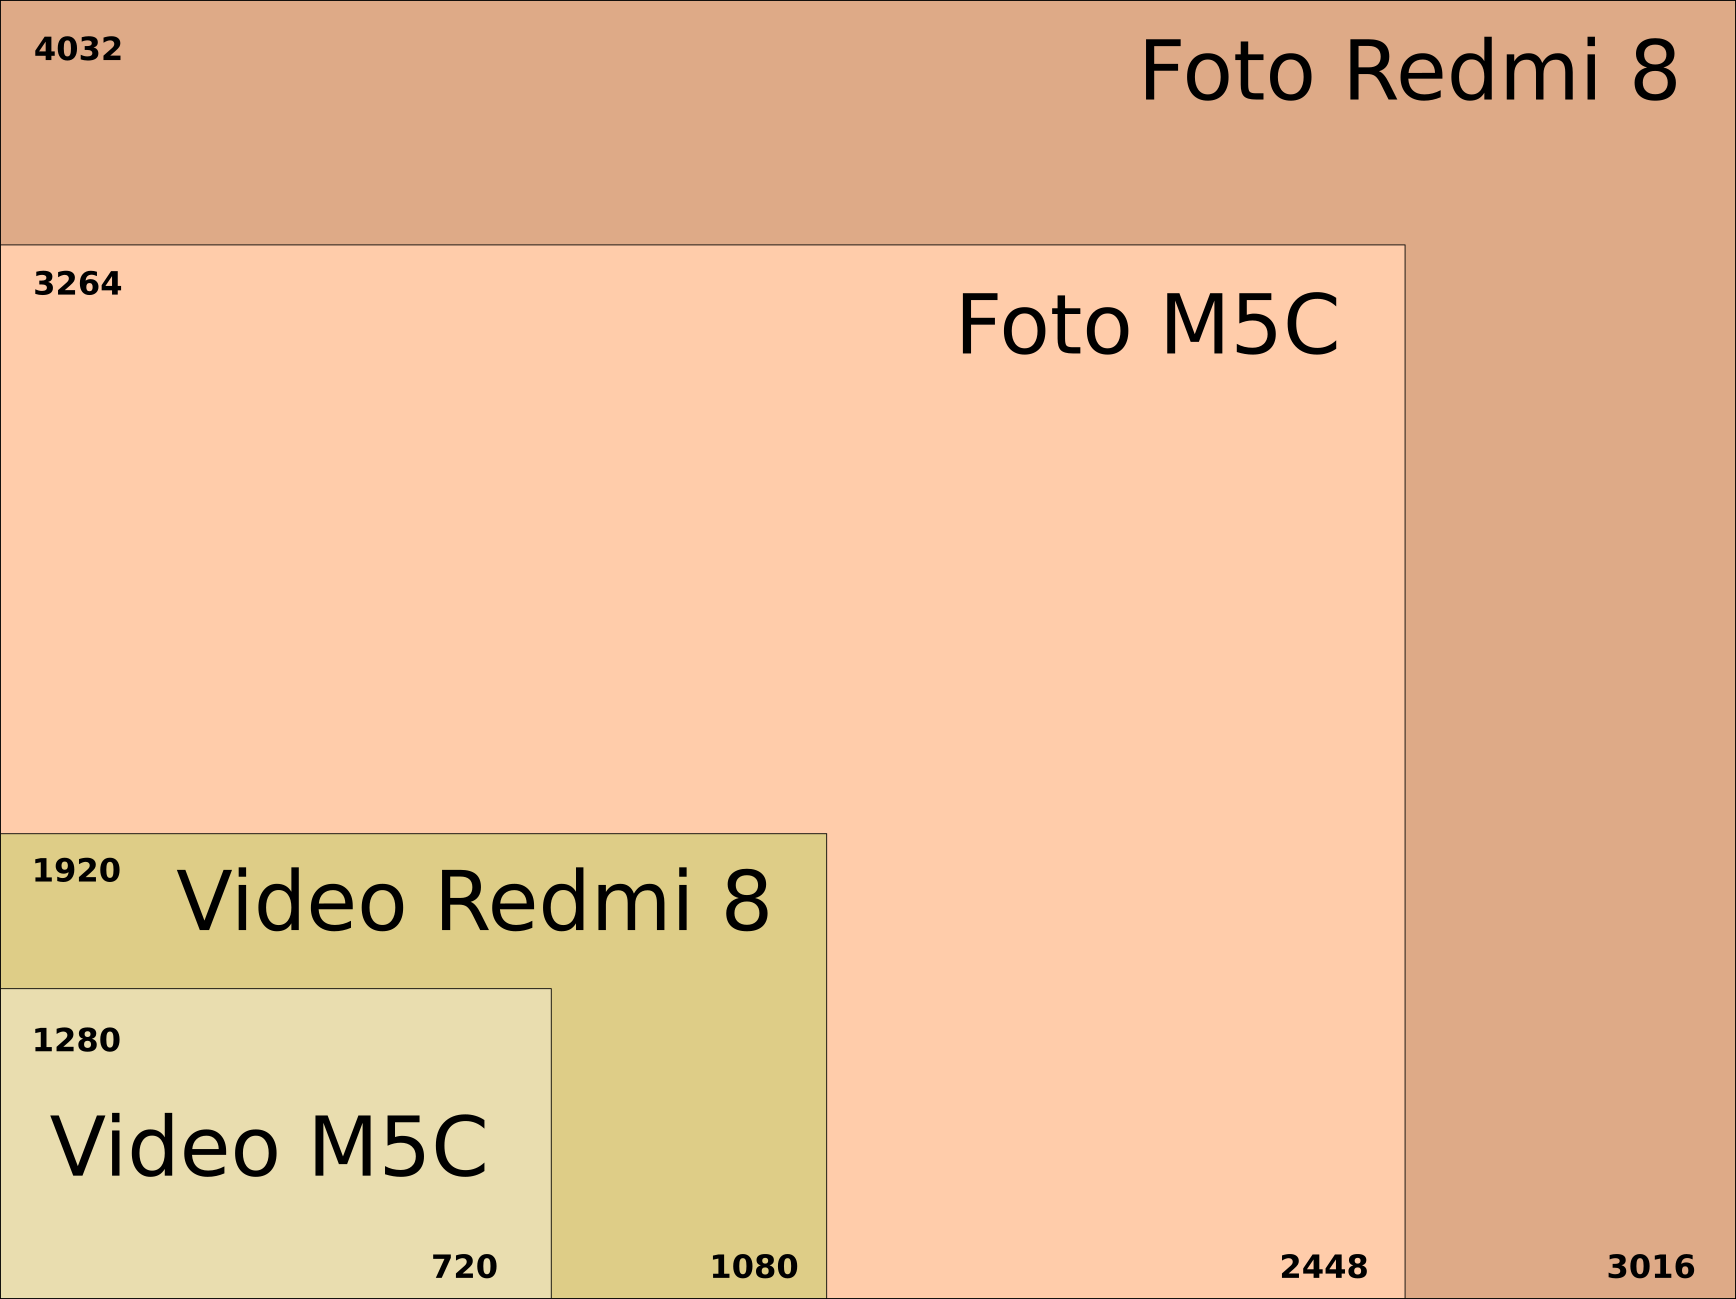
\includegraphics[width=0.6\textwidth,fbox]{figs/photo_video_dimensions.png}
   \caption{Comparativo de dimensões de foto e vídeo para os smartphones utilizados.}
   \label{fig:photo_video_dimensions}
\end{figure}
No modo vídeo o M5c produz imagens de 1280 x 720 pixeis, e o Redmi 8 produz imagens de 1920 x 1080 pixeis. Já no modo foto, o M5c produz imagens de 3264 x 2448 pixeis, e o Redmi 8 produz imagens de 4032 x 3016 pixeis. Após testes empíricos nos dois modos disponíveis, o modo vídeo no Redmi 8 apresentou o maior desempenho entre assertividade na identificação dos blocos e tempo de processamento.

O modo vídeo, entretanto, produz imagens em formato incompatível com exigido pela biblioteca TopCodes. Enquanto a TopCodes processa imagens em formato RGB\footnote{O RGB (\textit{Red, Green, Blue} - Vermelho, Verde e Azul) armazena as informações de cada pixel em 3 bytes, um para R, outro para G e outro para B. O valor de cada byte varia entre 0 e 255, onde 0 significa ausência de cor e 255 significa presença de cor. A cor preta é representada pela ausência das três cores, igual a 0 0 0, e cor branca é a presença total das três cores, igual a 255 255 255. Nesta estratégia cada um dos três bytes tem a informação de luminosidade.}, o formato gerado por vídeo é o YUV\footnote{Y significa luminosidade, e U e V representam intensidade das cores. Essa separação entre luminosidade e cores ocorreu por razões históricas. Os televisores em preto e branco necessitavam apenas da informação de luminosidade, e os televisores coloridos, que surgiram posteriormente, precisavam de canais de cores \cite{jack_video_2001}. O formato YUV manteve o funcionamento das televisões em preto e branco, que decodificavam apenas o canal Y, enquanto os aparelhos coloridos usaram também as informações de cores.
}. Portanto, é preciso converter o formato YUV para RGB, o que ocorre com a seguinte fórmula:

\begin{equation}
\label{equation:yuvrgb}
\centering
\begin{aligned}
R' &= Y + 1.140V \\
G' &= Y - 0.395U - 0.581V \\
B' &= Y + 2.032U
\end{aligned}
\end{equation}

A \autoref{equation:yuvrgb} precisa ser invocada para cada pixel. Para uma imagem de 1920 x 1080 isso significa iterar em um laço de repetição 2073600 vezes. Entretanto ess processo não ocorre apenas em uma imagem , mas sim em um fluxo contínuo de imagens.

Para que este tipo de processamento não cause atrasos perceptíveis para a interação do usuário, o módulo de câmera utiliza a API Renderscript. Essa api é um modo pelo qual o que o sistema Android viabiliza operações computacionais de alto desempenho, geralmente aplicado em processamento de imagens. O ganho de performance decorre da execução de código nativo, que pode ser e executado em modo paralelo na GPU \cite{sams_introducing_2011}. Isso viabiliza que mais e um píxel seja convertido simultâneamente.

\subsubsubsection{Módulo de Detecção de Blocos}

Após a captação da imagem e sua conversão para o formato RGB, o módulo de detecção de blocos processa as imagens a fim de identificar as marcas fiduciais. Os blocos são os objetos tangíveis que contém marcas fiduciais, apresentados na \autoref{fig:tangible_elements}. Este módulo utiliza a biblioteca TopCodes para facilitar a identificação dos objetos da cena. Esta biblioteca possui implementações nas linguagens Java, JavaScript e C++. O uso do algoritmo em Java se mostrou inviável devido à lentidão, restando o uso do algoritmo em C++. 

A tecnologia que viabiliza o uso de C++ em ambiente Android é \textit{Java Native Interface} (JNI). Para utilizar código nativo, uma função do tipo \mintinline{java}{external} é declarada no código Java ou Kotlin e sua implementação ocorre em C++. O \autoref{quadro:jni} demonstra o relacionamento entre ambas as linguagens. O código Kotlin invoca a função \mintinline{java}{external}, cuja implementação é em C++. Os parâmetros que transitam entre os dois ambientes são a altura e a largura da imagem, bem como uma lista de números inteiros que representam os pixeis da imagem no formato RGB.

\begin{quadro}[!h]
    \captionquadro{Ligação entre código nativo escrito e código Kotlin. }
    \begin{minted}[breaklines,frame=single]{kotlin}
    // kotlin (arquivo TopcodesScanner.kt)
    private external fun searchTopCodesNative(imageWidth: Int, imageHeight: Int, imageData: IntArray) : Array<TopCode>
    \end{minted}
    
    \begin{minted}[breaklines,frame=single]{c}
    // c++ (arquivo native-lib.cpp)
    extern "C" 
    JNIEXPORT jobjectArray JNICALL
    Java_topcodes_TopCodesScanner_searchTopCodesNative(JNIEnv *env, __unused 
    jobject _, jint image_width, jint image_height, jintArray image_data) 
    { 
        // uso da biblioteca topcodes em código nativo.
    }
    \end{minted}
    \label{quadro:jni}
\end{quadro}

Por fim, o código nativo retorna a lista de marcas detectadas. Cada marca tem como atributo a coordenada da marca, seu ângulo, tamanho e código identificador. Essas informações podem, então, ser analisadas para compreender o posicionamento dos elementos tangíveis no cenário.

\subsubsubsection{Módulo de Análise de Blocos}
Após a identificação dos blocos, o módulo de análise:

\begin{itemize}
\item analisa se um algoritmo foi construído
\item detecta o posicionamento do brinquedo RoPE sobre o tapete
\item detecta se o bloco ativador de depuração está visível
\end{itemize}

Estas ações são uma parte do código fonte propensa a mudanças. Outros blocos podem ser criados em funcionalidades futuras, exigindo análises específicas. A estrutura de código fonte deve considerar e evitar mudanças constantes em um mesmo arquivo, pois isso provoca o surgimento de erros e código difícil de manter. 
O padrão de projeto Composite foi a solução utilizada para evitar estes problemas. Esse padrão facilita a construção de hierarquias de objetos, construídas com grupos de objetos (composições) e objetos individuais (folhas). Tanto o tipo folha como composição obedecem uma mesma interface, e os objetos do tipo composição podem ter listas de folhas ou outras composições \cite{gamma_design_1994}.

\begin{figure}
\centering
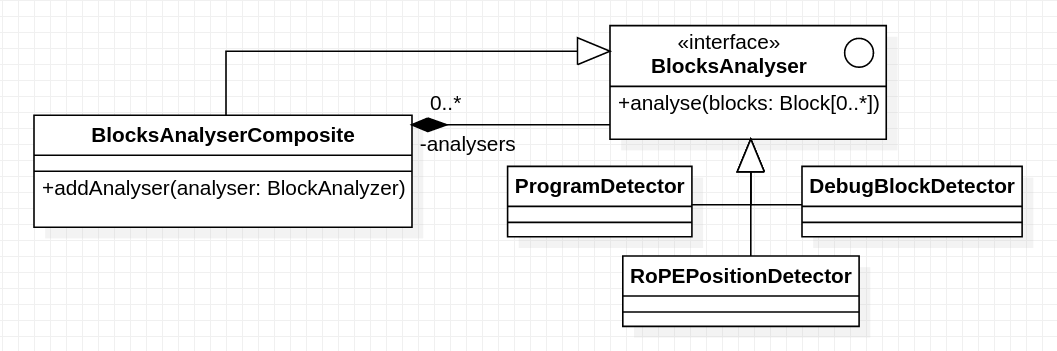
\includegraphics[width=0.8\textwidth,fbox]{figs/composite_diagram.png}
\caption{Aplicação do padrão Composite.}
\label{fig:composite}
\sourceauthor
\end{figure}

No código, o Composite viabiliza compor uma estrutura hierárquica que une analisadores de blocos. A \autoref{fig:composite} demonstra o uso do \textit{pattern}. A classe \mintinline{java}{BlocksAnalyserComposite} é uma composição, e as classes \mintinline{java}{ProgramDetector}, \mintinline{java}{RoPEPositionDetector} e \mintinline{java}{DebugBlockDetector} são folhas. Essas quatro classes implementam a interface \mintinline{java}{BlocksAnalyser}, ou seja, são analisadores de blocos. A primeira classe é um analisador composto pelos três analisadores folha.
O código cliente\footnote{Código que solicita a análise dos blocos.} tem apenas um objeto do tipo \mintinline{java}{BlocksAnalyserComposite}, o qual tem uma lista de analisadores. Quando o código cliente solicita a esse objeto que analise os blocos, este repassa a solicitação a cada um dos analisadores da lista para executarem especializadas (\autoref{quadro:composite}). O código cliente não sabe quais análises ocorrem, e o comportamento do programa pode ser alterado ao adicionar mais analisadores na composição. Isso evita alterações em cada um dos analisadores, que ficam responsáveis por ações específicas, e também evita alterações no código cliente, pois a interface com o composite se mantém inalterada.

\begin{quadro}[!h]
    \captionquadro{Implementação da classe de composição.}
    \begin{minted}[breaklines,frame=single]{kotlin}
    
    class BlocksAnalyzerComposite : BlocksAnalyzer {

        private val analyzers = mutableListOf<BlocksAnalyzer>()

        override fun analyze(blocks: List<Block>) {
            if(blocks.isNotEmpty()){
                // A composição repassa a solicitação de análise a cada um dos analisadores da sua lista.
                analyzers.forEach {
                    it.analyze(blocks)
                }
            }
        }

        fun addBlocksAnalyzer(analyser: BlocksAnalyzer) = analyzers.add(analyser)
        
    }
    \end{minted}
    \label{quadro:composite}
\end{quadro}


\subsubsubsection{Módulo de Registro de Interações - CtPuzzle Platform}
O módulo Log rastreia as interações do usuário e as armazena na plataforma web CtPuzzle Platform\footnote{\url{ctplatform.playerweb.com.br}}. Esta plataforma permite a criação de testes de Pensamento Computacional através da definição de \textbf{mecânicas} de jogos e desafios de lógica. Uma mecânica é um conjunto de atributos, que especificam de maneira abstrata as regras do jogo ou desafio. No caso desta pesquisa, o jogo ou desafio consiste em um mapa, com um caminho a ser percorrido, posições de objetos a serem coletado e um conjunto de comandos esperados como solução. 

Após a definição das mecânica do puzzle, a plataforma permite definir \textbf{itens} que correspondem à instâncias desse puzzle. Similar à fases de um jogo, cada item tem valores concretos de acordo com o que as definições da mecânica\footnote{Pode-se comparar mecânica e item com classe e objeto, na programação orientada a objetos. A classe/mecânica define atributos, e o objeto/item tem valores concretos para estes atributos.}.  Neste trabalho, a mecânica define o puzzle deve ter objetos coletáveis, que o robô deve capturar. Um item especifica que haverá um objeto na posição (2,3) do mapa, e que este mapa terá uma dimensão de 4 por 5. O aplicativo implementa a interface do jogo com base nestas regras. Ao todo são 9 itens, cada um com um caminho e uma maçã a ser capturada. 

Estes itens são por fim agrupados e sequenciados formando uma sequência de fases de um jogo.

Por fim, o aplicativo envia para a plataforma as respostas para cada um dos itens testados, ou seja, para cada fase. Cada resposta possui uma lista de tentativas de solução do desafio, que são os algoritmos executados pelo robô. Isso permite entender como as estratégias de resolução mudaram até a obtenção da solução.

\subsubsection{RoPE: Comunicação Bluetooth}
Para entender como ocorre a comunicação com o brinquedo RoPE via Bluetooth é necessário entender a organização do seu \textit{firmware} e o conceito de comunicação serial. O \textit{firmware} é o programa instalado no chip ATMega3268p, o qual é acoplado à placa principal e coordena as reações aos eventos percebidos pelo brinquedo. As reações possíveis são o acionamento de  luzes, o acionamento dos motores e a emissão de sons. O \textit{firmware} coordena o acionamento dessas ações em eventos de cliques nos botões e de recepção de mensagens na comunicação serial do Arduino.

A comunicação serial possibilita a transferência de dados entre uma placa Arduino e outros computadores ou dispositivos. Todas as placas Arduino possuem ao menos dois pinos para essa comunicação, sendo um para leitura e outro para a escrita. Normalmente a comunicação ocorre por cabos para a transferência de código hexadecimal, o qual gerado em ambientes de desenvolvimento e transferido para a placa para atualização do \textit{firmware}.

Além disso, esses mesmos pinos permitem a comunicação sem fio por Bluetooth ou Wi-Fi por meio da adaptação de módulos. Os módulos são dispositivos de hardware com funcionalidades específicas, não encontradas por padrão em placas Arduino. Um destes módulos é HM-10, destinado a habilitar comunicação Bluetooth de baixo consumo de energia (BLE - \textit{Bluetooth Low Energy}). Esse módulo possui os pinos de energia (VCC), aterramento (GND), leitura (RX) e escrita (TX). Os pinos de leitura e escrita são conectados aos pinos de escrita e leitura do brinquedo RoPE, o que habilita a transferência de dados recebidos via Bluetooth pelo módulo, o qual os repassa via serial para o chip do brinquedo (\autoref{fig_connection_hm10}).

\begin{figure}[!h]
    \centering
    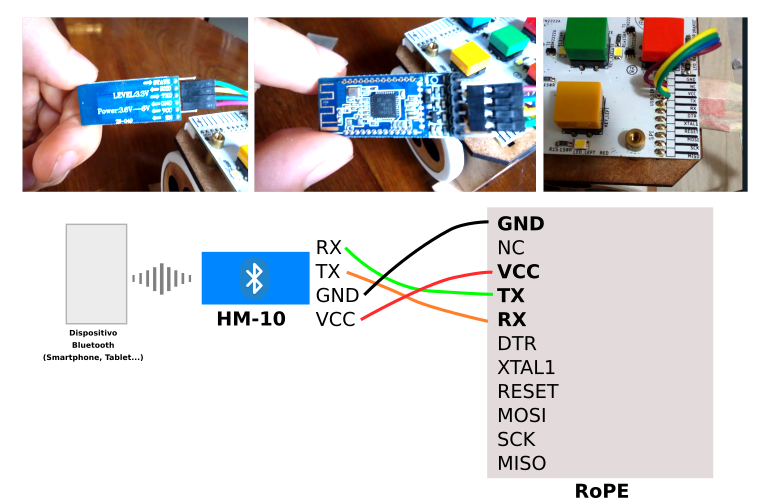
\includegraphics[width=.8\linewidth,fbox]{figs/connection_rope_hm10.png}
    \caption{Conexão entre o módulo HM-10 e a placa do brinquedo RoPE.}
    \label{fig_connection_hm10}
    \sourceauthor
\end{figure}

O \textit{firmware} é responsável por interpretar os dados recebidos na serial. Este é implementado seguindo o paradigma de Orientado a Objetos, a fim de mapear as responsabilidades e componentes físicos existentes no brinquedo. Neste sentido, o código fonte do \textit{firmware} tem classes que correspondem aos componentes de \textit{hardware} como buzzer, CPU, teclado e bateria. A classe \textit{Battery}, por exemplo, monitora o nível da bateria e impede o acionamento do brinquedo quando há pouca energia armazenada.

\begin{figure}[!ht]
    \centering
    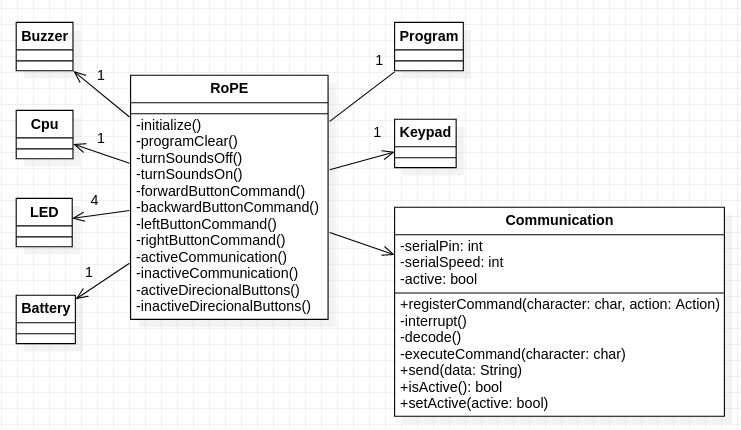
\includegraphics[width=.8\linewidth,fbox]{figs/class_diagram_firmware.png}
    \caption{Diagrama de classes do firmware.}
    \label{fig:classes_firmware}
    \sourceauthor
\end{figure}

Seguindo este paradigma, este trabalho adicionou ao código existente uma classe responsável pela comunicação, ou seja, recepção, interpretação e envio de dados por meio da comunicação serial. Essa classe de comunicação permite o registro de caracteres que, ao serem captados, acionam funcionalidades oferecidas pelo brinquedo. A recepção da letra \textit{f}, por exemplo, dispara a ação \textit{adicionar o comando "frente" na sequência de ações}.

Um protocolo de comunicação define os caracteres a serem enviados, bem como uma sequência de caracteres para definir o início de uma mensagem (\autoref{quadro:protocol}). Além disso, o protocolo define mensagens que informam eventos ocorridos no brinquedo, de modo que aplicações externas possam refletir mudanças de estado, como por exemplo destacar um bloco de código em execução.
{\renewcommand{\arraystretch}{1.3}
\begin{quadro}
    \caption{Protocolo de comunicação}
    \label{quadro:protocol}
    \begin{centering}
    \begin{tabular}{|p{.3\textwidth}|p{.6\textwidth}|}
        \hline
        \multicolumn{2}{|c|}{\textbf{Mensagens externas para o RoPE}} \\ \hline
        String           & Ação do RoPE                                \\ \hline
        cmds:            & Indica início de mensagem \\ \hline
        c                & Apaga o programa da memória \\ \hline
        s                & Desativa sons \\ \hline
        S                & Ativa sons \\ \hline
        f                & Adiciona comando "frente" no programa \\ \hline
        b                & Adiciona comando "trás" no programa \\ \hline
        r                & Adiciona comando "direita" no programa \\ \hline
        l                & Adiciona comando "esquerda" no programa \\ \hline
        e                & Executa programa \\ \hline
        a                & Desativa conexão Bluetooth \\ \hline
        x                & Desativa botões direcionais \\ \hline
        X                & Ativa botões direcionais \\ \hline
        \multicolumn{2}{|c|}{\textbf{Mensagens do RoPE para outros dispositivos}} \\ \hline
        Expressão regular & Mudança de estado do brinquedo \\ \hline
        <addi:(f|b|r|l)>  & Comando "frente", "trás", "direita" ou "esquerda" adicionado \\ \hline
        <start\_required>  & Botão "iniciar" pressionado e o brinquedo está em estado de programação externa \\ \hline
        <program:(started|terminated)>  & Notifica início e término de execução. \\ \hline
        <executed:[0-9]{1,2}>  & Notifica início da execução de um comando. \\ \hline
    \end{tabular}
    \end{centering}
    \sourceauthor
\end{quadro}
}


Ao registrar funções disparadas quando do recebimento de caracteres, o código usa o padrão \textit{Observer} \cite{gamma_design_1994}, o que facilita registrar novos caracteres para alterar o comportamento do robô. A limitação do registro de apenas um caractere é que uma letra apenas identifica a função a ser invocada, mas não informa seus parâmetros. Para isso seria necessário o envio de uma letra para identificar a função a ser invocada, seguida de uma lista de valores a serem inseridos nesta função. Essa funcionalidade não foi implementada pois a passagem de parâmetros não é um requisito da aplicação atual.

\begin{quadro}[!h]
\caption{Ligação entre caracteres e funções executadas no brinquedo.}
    \begin{footnotesize}
    \fbox{
        \begin{minipage}{1\textwidth}
      
            {\fontfamily{qcr}\selectfont
                communication.registerCommand('c', programClear);\\
                communication.registerCommand('s', turnSoundsOff);\\
                communication.registerCommand('S', turnSoundsOn);\\
                communication.registerCommand('f', forwardButtonCommand);\\
                communication.registerCommand('l', leftButtonCommand);\\
                communication.registerCommand('r', rightButtonCommand);\\
                communication.registerCommand('b', backwardButtonCommand);\\
                communication.registerCommand('a', inactiveCommunication);\\
                communication.registerCommand('A', activeCommunication);\\
                communication.registerCommand('x', inactiveDirectionalButtons);\\
                communication.registerCommand('X', activeDirectionalButtons);\\
                communication.registerCommand('e', executeButtonExternalAction);\\
            }
    
        \end{minipage}
    }
    \end{footnotesize}
\end{quadro}

\section{Considerações}

Este capítulo descreveu os elementos da interface RoPE AR. Iniciou apresentando os elementos com os quais o usuário interage, que é o aplicativo para Android e os elementos tangíveis. A seguir 